\documentclass[12pt,lot,lof]{puthesis_undergraduate}
\usepackage{amsfonts}
\usepackage{amssymb}
\usepackage{amsmath}
\usepackage{amsthm}
\usepackage{latexsym}
\usepackage{graphicx}
\usepackage{physics}
%\usepackage{setspace}
%\usepackage[round, longnamesfirst]{natbib} % for nice bibliography

%%%%%% ENVIRONMENTS %%%%%%
%\swapnumbers
%\newtheorem{theorem}{Theorem}
%\newtheorem{proposition}[theorem]{Proposition}
%\newtheorem{lemma}[theorem]{Lemma}
%\newtheorem{definition}[theorem]{Definition}
%\newtheorem{corollary}[theorem]{Corollary}
%\newtheorem{remark}[theorem]{Remark}
%\newtheorem{conjecture}[theorem]{Conjecture}
%\newtheorem{notation}[theorem]{Notation}
%\newtheorem{example}[theorem]{Example}
%\newtheorem{exercise}{Exercise}
%\newtheorem*{notes}{Notes}

% For PUthesis.cls use the following definitions:
\newtheorem{theorem}{Theorem}[section]
\newtheorem{lemma}[theorem]{Lemma}
\newtheorem{corollary}[theorem]{Corollary}
\newtheorem{proposition}[theorem]{Proposition}
\newtheorem{definition}[theorem]{Definition}
\newtheorem{claim}{Claim}
\newtheorem{conjecture}[theorem]{Conjecture}
\newtheorem{observation}[theorem]{Observation}
\newtheorem{problem}[theorem]{Problem}



%%%%%% NEW COMMANDS/OPERATORS %%%%%%
\DeclareMathOperator{\esup}{\text{ess\;sup}}
\providecommand{\abs}[1]{\lvert#1\rvert} % absolute value function
\renewcommand{\P}{\mathbb{P}}  % probability measure
\renewcommand{\O}{\mathcal{O}} % order notation
\newcommand{\PP}{\P^\star} % pricing probability measure
\newcommand{\E}{\mathbb{E}}  % expectation
\newcommand{\Var}{\mathrm{Var}}
\newcommand{\EE}{\E^\star}   % expectation under the pricing measure
\newcommand{\V}{\text{Var}} % variance
\newcommand{\F}{\mathcal{F}} % filtration
\newcommand{\G}{\mathcal{G}} % filtration
\renewcommand{\H}{\mathcal{H}} % filtration
\newcommand{\Fb}{\mathbb{F}} % filtration
\newcommand{\N}{\mathbb{N}}  % integers
\newcommand{\R}{\mathbb{R}}  % real numbers
%\renewcommand{\C}{\mathbb{C}}  % complex numbers
\newcommand{\argmin}{\mathop{\mathrm{arg\,min}}} % arg min operator
\newcommand{\cpb}{c^{\mbox{\scriptsize pb}}} % protection buyer payment
\newcommand{\cps}{c^{\mbox{\scriptsize ps}}} % protection seller payment
\newcommand{\cds}{c^{\mbox{\scriptsize ds}}} % CDS spread

\newcommand{\T}{\mathcal{T}} % tenor
\renewcommand{\vec}[1]{\mbox{\boldmath $#1$}} % boldface 1 for the indicator function
\newcommand{\ind}{\vec{1}}                    % boldface 1 for the indicator function
\newcommand{\Ws}{W^\star_t}
\newcommand{\tWs}{\widetilde{W}^\star_t}
\newcommand{\tWz}{\widetilde{W}^0_t}
\newcommand{\tW}{\widetilde{W}}

%%%%%% Shortcut expressions %%%%%%
%\newcommand{\pb}{protection buyer}
\newcommand{\ps}{protection seller}
\newcommand{\BibTeX}{{\sc Bib}\TeX}

%%%%%% Greeks %%%%%%
\newcommand{\eps}{\varepsilon}
\newcommand{\de}{\delta}
\newcommand{\fee}{\varphi}
\newcommand{\half}{\frac{1}{2}}

%%%%%% PDEs %%%%%%%
\newcommand{\pa}{\partial}
\renewcommand{\L}{\mathcal{L}}
\newcommand{\M}{\mathcal{M}}
\newcommand{\A}{\mathcal{A}}
\newcommand{\wA}{\widetilde{\A}}
\newcommand{\wlop}{\widetilde{\L}}
\newcommand{\wmop}{\widetilde{\M}}
\newcommand{\lbs}{\L_{BS}}
\newcommand{\lbss}{\L_{BS^\star}}
\newcommand{\lzero}{\L_{0}}
\newcommand{\lone}{\L_{1}}
\newcommand{\ltwo}{\L_{2}}
\newcommand{\wled}{\widetilde{\L}^{\eps,\de}}
\newcommand{\wlone}{\widetilde{\L}_1}
\newcommand{\wltwo}{\widetilde{\L}_2}
\newcommand{\cltwo}{\langle \L_2 \rangle}
\newcommand{\cwltwo}{\left\langle \wltwo \right\rangle}
\newcommand{\mone}{\M_{1}}
\newcommand{\mtwo}{\M_{2}}
\newcommand{\mthree}{\M_{3}}
\newcommand{\wmone}{\widetilde{\M}_1}
\newcommand{\fc}{\langle f \rangle}  % <f>

\newcommand{\bes}{\begin{equation*}}

%%%%%% OLD ONES %%%%%%
%\newcommand{\sigbar}{\overline{\sigma}}
%\newcommand{\sigstar}{\sigma_\star}
%\newcommand{\CBS}{C_{BS}}
%\newcommand{\CBSs}{C_{BS^\star}}
%\newcommand{\BS}{Black-Scholes }
%\newcommand{\vol}{volatility}
%\newcommand{\SV}{stochastic volatility }
%\newcommand{\PP}{{\mathord{I\kern -.33em P}}}
%\newcommand{\EE}{{\mathord{I\kern -.33em E}}}
%\newcommand{\RR}{{\mathord{I\kern -.33em R}}}
%\newcommand{\1}{{\mathord{1\kern -.26em \text{I}}}}
%\newcommand{\calp}{{\PP}}
%\newcommand{\EEE}{{\EE^{\star}}}
%\newcommand{\PPP}{{\PP^{\star}}}
%\newcommand{\ssb}{\overline{\sigma^2}}



\title{Systematic Analysis in Three-Dimensional Reconstruction of Weak-Lensing Mass Maps
with a Sparsity Prior}
\submitted{May 2023}  %graduation date
\author{Shouzhuo Yang}
\advisor{Naoki Yoshida} %
\dedication{}


\abstract{
\begin{enumerate}
\item cosmology basics... $\Lambda CDM$. A little bit of FDR metric...
\item Dark Matter halos. virialization... growth of perturbations. Different kinds of dark matter halo. Describe very briefly different dark matter prediction of dark matter halo profiles.
\item Weak lensing basics. Some Newtonian/GR level calculation. What can the weak lensing probe about our universe. 
\item Weak lensing systematics. This is the part I am worst at.. I will need to ask Yoshida about whether to write about it. Weak lensing noise is something I definitely should mention. 
\item Sparsity analysis
\item 3d mass reconstruction (including a mention of other reconstruction research). 
\item results? 

\end{enumerate}
}

\acknowledgements{
I wish to first give my heartfelt gratitude toward the Department of the Physics and Astronomy for hosting the honors program and provide me this opportunity to summarize my work in weak lensing cosmology. It has been truly a satisfying process.
My thanks also goes to Professor Tristan Smith for setting up this project with Professor Naoki Yoshida, who offered me a wonderful journel of cosmology. 
Also, I wish mention my collaborator and friend Xiangchong Li from Carnegie Mellon University who helped me not only with this project but various aspect on physics. 
I appreciate the help also of my two other research advisors, Peter Collings and Michael Brown, for supporting my thesis in their own way. 
Finally, I wish to thank my partner Meihan ``Della'' Guo, who, though not contributing scientifically, provided me emotional support that have gotten me through the project. 

}

\begin{document}
\chapter{Introduction}\label{ch:intro}  %insert chapter title

Hello World. See \cite{A01}.

See \cite{A01} and \cite{ARS03} for more information.

This is the introduction of my sample thesis. Let me just state that
this is a very, very limited introduction to \LaTeX, and I can not
do justice to it through the next few pages.

I recommend reading this .pdf file along with the .tex file open on
the side so that you can compare the pure ASCII text and the final
result after compilation.

\section{A Different Word Processing System} \label{ch:anotherintro}
I highly recommend the booklet ``The Not So Short Introduction to
\LaTeXe{}'' which is free and very well-written. It is available on:
\begin{center}
\verb|http://tobi.oetiker.ch/lshort/lshort.pdf|.
\end{center}

\noindent I refer you to the introduction there.

 % and path to the .tex file (no need to include .tex)

\chapter{Development of the Department of Operations Research and Financial Engineering}  %continue adding chapter titles
%%% This is the development.tex

This Chapter has purposefully a very long title to illustrate how
\LaTeXe{} handles such long names. Now it is a good time to look on
the table of contents and see how this Chapter and also
Chapter~\ref{ch:intro} are listed. Notice that the number 1 in the
phrase ``and also Chapter 1'' is automatically generated by using
the command \verb|\ref{ch:intro}|, because we labeled
Chapter~\ref{ch:intro} `\verb|ch:intro|' by using the command
\verb|\label{ch:intro}| after the \verb|\chapter{Introduction}|
declaration.

\section{Initial Setup}
A few things here to start. And here as well, since we need to fill
in at least a line. Almost\ldots, there we go!

Notice that I entered ellipses after the word `Almost' above with
the command \verb|\ldots|, and not by simply typing three dots.
Compare the result here: \ldots vs. ...\footnote{Word does that too,
but lousily!}

Maybe some more words in a new paragraph. And more, and more, and
more. Furthermore, additionally, in addition, and so on. Notice here
that the word `Furthermore' was broken into `Fur-' and `thermore' in
order to fit the line---Word, as stupid as it is, would simply place
the entire word on the next line, thus increasing the distance
between words on the first line to fill up the entire line.

\subsection{Additional Structure: The Use of Subsections}
\label{sec:structure} We are in a subsection now (two levels down
from a Chapter). When we refer to $X.Y.Z$, we mean Chapter $X$,
Section $Y$, and subsection $Z$. We declare a Chapter by the command
\verb|\chapter{|\emph{title of Chapter}\verb|}|, a Section by
\verb|\section{|\emph{title of Section}\verb|}|, and so on.

The nice thing about \LaTeX{} is that it takes care of the chapter,
section, and subsection numbering automatically. If I were to add
another subsection before this one the subsection number would
change (increment by one). This section is \ref{sec:structure} and I
referred to it using the command \verb|\ref{|\emph{label of this
section}\verb|}|. I inserted a label right after the
\verb|\subsection| declaration by typing \verb|\label{|\emph{label
of this section}\verb|}|.

\subsubsection{A subsubsection}\label{subsub} Just for fun! Notice
that no number is alloted for such a low level environment but it
sometimes useful.

\subsection{Another Subsection}
And so on\ldots.

\section{Mathematical Symbols}
Let $X=\{X_n, n\in \N\}$ be a Markov chain with state space
$\mathcal{D}$. Throughout this thesis, we use the notation
\begin{equation}
p_{ij} := \P\{X_{n+1} = j \mid X_n = i\}, \quad i,j \in \mathcal{D}
\label{pij}
\end{equation}
for the transition probabilities of the Markov chain $X$.
Furthermore, we denote by $P$ the transition matrix, $P =
[p_{ij}]_{i,j\in\mathcal{D}}$.

When we wrote \eqref{pij} we implicitly assumed that the Markov
chain $X$ is time-homogeneous.

Let us also define $Y$,
\begin{equation*}
Y = (Y_n)_{n = 0,1,2,\ldots}
\end{equation*}
to be another process. Notice that the second equation does not take
a number on the right---this is the use of \verb|\begin{equation*}|
environment.

Notice that the all the math characters, $X$, $\mathcal{D}$, and
others such as $\alpha, \beta, \gamma$ are part of the text in
\LaTeX{}. On the contrary, Word includes such characters as foreign
objects (usually images), which increases the size of the document
file, sometimes makes them disappear, but most importantly are not
as aesthetically pleasing as the resulting characters here.

\section{Citing and Bibliography}
When working with large documents you need an easy way to cite your
references without having to go back to your list all the time to
remember the names of the authors and the year of publication. Even
more importantly, you need to have all your references listed in the
end of the document in alphabetical order. Of course, they all need
to be syntactically the same so that alone makes the manual entry of
references a big pain. Thankfully, \LaTeX{} takes care of that in a
very easy and elegant way, using \BibTeX.

I cite here a few books, papers, and technical reports, and please
go to page \pageref{bib} to see the resulting bibliography.

According to the books by \cite{C75}, \cite{BR02}, and \cite{MR97}
and the articles by \cite{DG01}, \cite{BBM05}, and \cite{CFPS04} we
conclude absolutely nothing. However, in his report, \cite{A04}
claims that otherwise. All these citations were entered by \verb|\cite{|\emph{citation label}\verb|}|.
 
Notice the different citation style that follows: it is parenthetical, and observe that only one pair of parentheses is required \cite[see Theorem 5.2 on pg. 32]{AMM05}. This citation is entered by typing \verb|\cite[see Theorem 5.2 on pg. 32]{AMM05}| in the \verb|.tex| file. (Here, the citation label corresponding to \cite{AMM05} is obviously \verb|AMM05|.)

The citations are included in the file \verb|refs.bib| under the
folder \verb|Bibliography|. You can modify it and make your own
references.

Also notice that \LaTeX{}, by default, includes in the Bibliography section only the references you actually cited throughout the text. If you want a source to appear in the Bibliography section without actually citing it anywhere in your text use the command \verb|\nocite{|\emph{citation label}\verb|}|. For example here I type \verb|\nocite{B95}| \nocite{B95} and you see no citation appear---however look at the fourth entry of the Bibliography. That cited book does not appear anywhere in this thesis, other than the Bibliography.

\section{Referencing Figures and Tables}
The very informative Figure~\ref{fig:dens} is on page~\pageref{fig:dens}. Both of these numbers were automatically generated---which is great when you add a new figure before the one you just inserted, because the numbering changes automatically for you. Use \verb|\ref{fig:dens}| for the figure number and \verb|\pageref{fig:dens}| for the page number where the figure is located. Here, \verb|fig:dens| was the label of the figure (see actual \verb|.tex| file for more information). Remember that \LaTeX{} does not work like Word---the figures and tables are \textbf{not} always placed exactly where you want them, so avoid writing ``according to the figure below\ldots,'' and prefer writing ``according to Figure~[\emph{figure number}]\ldots,'' instead. The same things go unchanged for tables. Notice that when I talk about figures and tables in general, I do not need to capitalize them, however if I talk specifically about Figure~\ref{fig:dens} and Table~\ref{tab:cdo}, I'd better respect them and capitalize the `f' and the `t.'

Since we're at it, notice that the quotes `, ', ``, '' are not inserted like in Word. For ` you need to use the \verb|`| key that is located above the \verb|Tab| button. For ' you just press the \verb|'| key, exactly to the left of the \verb|Enter| key. For double quotes just double the appropriate single quotes without leaving any space.

\section{Introduction to Sparisty Analysis}

Given the prevalence and the strength of noise in weak lensing analysis, to successfully reconstruct physical information from weak lensing data, one may be prompted to use \emph{sparsity}. A \emph{sparse} model indicates only a relatively small amount of parameters controls
the behavior of the system. In weak lensing and specifically 3D reconstruction, we apply this idea to assert that galaxy clusters are only sparsely 
distributed in the present universe. 

To implement the sparisty prior in an analysis, first consider the familiar linear regression model: 

\begin{equation}
  y_i = \beta_0 + \sum^{p}_{j=1} x_{ij}\beta_j + e_i
\end{equation}
where $\beta_0$ and $\beta = (\beta_1, \beta_2, \ldots, \beta_p)$ are unknown multidimensional linear parameters of some model. $y_i$'s are measured values, and $e_i$'s are errors of estimation.

To retrieve the best predicted model, one acquire an estimation of $\beta$ parameters by mininizing the least-squares objective function. 
\begin{equation}
  \mathrm{minimize}_{\beta, \beta_0} \sum^N_{i=1}(y_i - \beta_0 - \sum^{p}_{j=1}x_{ij}\beta_j)^2
\end{equation}

However, when the number of undertermined parameters is large, such an objective function may yield nonzero value for the $\beta$ vector and yield degenerate solutions. This makes the interpretation of the result difficult. 
A solution is just to \emph{regularize} the estimation process. The regime we will be working with in this work is called the Lasso regularization, which uses the Lasso Estimator:

\begin{equation}
  \mathrm{minimize}_{\beta_0, \beta}\{\frac{1}{2N} \sum^N_{i=1}(y_i-\beta_0 - \sum^{p}_{j=1}x_{ij}\beta_j)^2\}
\end{equation}
subject to 
\[\lVert \beta \lVert_1\leq t.\]
Where $\lVert \beta \lVert_1$ represents the $l_1$-norm which is the sum of the absolute values of each entries in $\beta$. 

In matrix form, one may have
\begin{equation}
  \mathrm{minimize}_{\beta_0, \beta}\Bigl\{\frac{1}{2N} \lVert \bf{y} - \beta_0 \bf{1} - \bf{X}\beta\lVert^2_2\Bigl\}
\end{equation}

subject to 
\[\lVert \beta \lVert_1\leq t.\] 

One can also rewrite this into the Lagrangian form
\begin{equation}
  \mathrm{minimize}_{\beta\in \mathbb{R}^p}\Bigl\{ \frac{1}{2N}\lVert \bf{y} - \bf{X}\beta \lVert^2_2 + \lambda \lVert\beta \lVert_1\Bigl\}
\end{equation}

Here then $\lambda \geq 0$ now controls the degree of sparisty we impose on the minimization, with larger $\lambda$ correspond to stronger sparse condition. 
\chapter{Analysis of Problem}
%% This is the analysis.tex file

Time for some analysis, and probably graphs and tables. Thankfully
\LaTeX{} (and \LaTeXe{}) provides very nice environments for both.

\section{Preliminary Analysis}
\begin{figure}[t]
\begin{center}
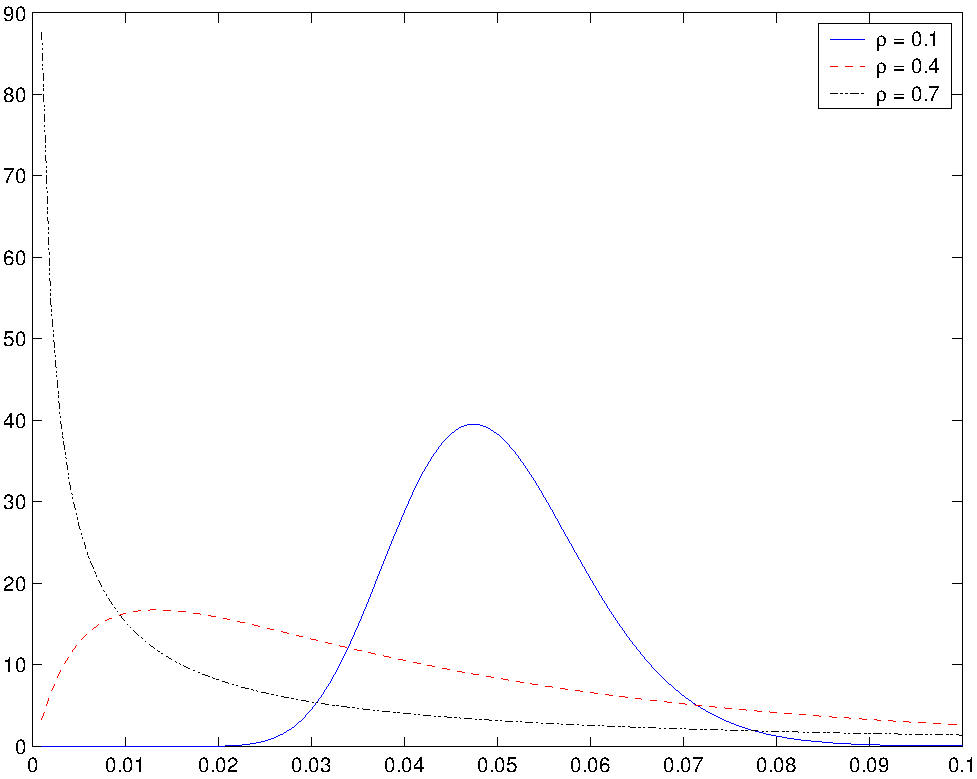
\includegraphics[width=0.8\textwidth]{./Figures/dens.pdf}
\caption{The density function $f$ as given in \eqref{density} for
  three different $\rho$'s and $\bar{p} = 0.05$. (Plotted on $[0,
  0.1]$ for convenience.)}
\label{fig:dens}
\end{center}
\end{figure}
Assume that the random variable $D$ given $\tilde{p} = p$ is
binomially distributed with parameters 50 and $p$ (probability of
success, in this case default). We also take the cumulative
distribution function of $\tilde{p}$ to be
\begin{equation*}
F(\theta) = \P\{\tilde{p} \le \theta\} = \Phi \left( \frac{1}{\rho}
\left(\sqrt{1 - \rho^2}\, \Phi^{-1}(\theta) - \Phi^{-1}(\bar{p})
\right) \right)
\end{equation*}
where $\Phi$ is the cumulative standard normal distribution
function, $\rho$ is the correlation coefficient between the
idiosyncratic and market factors and $\bar{p}$ is the mean default
probability ($\bar{p} = \E \tilde{p}$). To calculate the density of
$\tilde{p}$ let
\begin{eqnarray*}
h(\theta, \rho, \bar{p}) &:=& \frac{1}{\rho} \left(\sqrt{1 -
\rho^2}\, \Phi^{-1}(\theta) - \Phi^{-1}(\bar{p}) \right), \\
\varphi(\theta) &:=& \frac{d}{d \theta} \Phi(\theta) =
\frac{1}{\sqrt{2 \pi}} e^{- \theta^2/2},
\end{eqnarray*}
and notice that since $\Phi$ is a bijection we have
\[\Phi \circ \Phi^{-1}(\theta) = \Phi^{-1} \circ \Phi(\theta) =
\theta, \] for every $\theta \in \R$. Then, we have for the density
of $\tilde{p}$,
\begin{eqnarray}
f(\theta, \rho, \bar{p}) &=& \frac{d}{d \theta} F(\theta) =
\Phi'(h(\theta, \rho, \bar{p})) \frac{\pa}{\pa \theta} h(\theta,
\rho, \bar{p}) \nonumber \\
&=& \varphi(h(\theta, \rho, \bar{p})) \frac{\sqrt{1 -
\rho^2}}{\rho} \frac{d}{d \theta} \Phi^{-1}(\theta) \nonumber \\
&=& \varphi(h(\theta, \rho, \bar{p})) \frac{\sqrt{1 - \rho^2}}{\rho}
\frac{1}{\varphi (\Phi^{-1}(\theta))}, \label{density}
\end{eqnarray}
for $\theta \in (0,1)$ and zero otherwise, since
\begin{eqnarray*}
\frac{d}{d \theta} \left(\Phi (\Phi^{-1}(\theta)) \right) &=&
\Phi'(\Phi^{-1}(\theta)) \frac{d}{d \theta} \Phi^{-1}(\theta)
\Leftrightarrow \\
\frac{d}{d \theta} \theta &=& \varphi(\Phi^{-1}(\theta))
\frac{d}{d \theta} \Phi^{-1}(\theta) \Leftrightarrow \\
\frac{d}{d \theta} \Phi^{-1}(\theta) &=&
\frac{1}{\varphi(\Phi^{-1}(\theta))}.
\end{eqnarray*}



The density of $\tilde{p}$ is shown in Figure \ref{fig:dens} for
three different values of $\rho$ and $\bar{p} = 0.05$. The effect of
the correlation is to put more mass towards higher default
probabilities as the correlation increases, thus resulting in larger
number of defaults as the correlation increases.

\begin{table}[htbp]
\caption{Values of the CDO Tranches.} \label{tab:cdo}
\begin{center}
\begin{tabular}{lllll}
\hline \hline
&            &             \multicolumn{ 3}{c}{$\rho$} \\
\hline
&            &       0.1 &        0.4 &        0.7 \\
\hline Equity &        $C_E^\star(T)$ &     2.5712 &     2.8957 &
3.5642 \\
Junior &        $C_J^\star(T)$ &     9.9289 &     9.6137 &
9.2120 \\
Senior &        $C_S^\star(T)$ &    35.0000 &    34.9905 &
34.7239 \\
\hline Sum & $C_E^\star(T) + C_J^\star(T) + C_S^\star(T)$ & 47.5000&
47.5000 &  47.5001 \\
\hline \hline
\end{tabular}
\end{center}
\end{table}
Using the default values for the parameters as above we get the
values for the tranches in Table~\ref{tab:cdo}.

Let's see one more result on Table~\ref{tab:cdo}. According to\ldots


\appendix
\chapter{Code}
%% Code file

\begin{verbatim}
% Question 1
warning('off'); % To protect our nerves
p = 0.05;
K_E = 5;
K_J = 10;
K_S = 35;

tmp1 = [];
for i = 0:(K_E-1)
     tmp1(i+1) = (K_E - i) * binopdf(i,50,p);
end
C_E = sum(tmp1)

tmp2 = [];
for i = (K_E+1):50
    tmp2(i-K_E) = (i-K_E) * binopdf(i,50,p);
end
tmp3 = [];
for i = (K_E + K_J +1):50
    tmp3(i- K_E - K_J) = (i - K_E - K_J) * binopdf(i,50,p);
end
C_J = K_J - sum(tmp2) +sum(tmp3)

C_S = K_S - sum(tmp3)

% Sanity check
C_E + C_J + C_S
\end{verbatim}



\bibliographystyle{abbrv}
\bibliography{refs} \label{bib}


\end{document}
